\documentclass{article}
\usepackage[utf8]{inputenc}
\setlength{\parskip}{1em}


\title{Chapter 3}
\author{jaynaythan }
\date{October 2019}

\usepackage{natbib}
\usepackage{graphicx}

\begin{document}

\maketitle

\section{Introduction}
There is a theory which states that if ever anyone discovers exactly what the Universe is for and why it is here, it will instantly disappear and be replaced by something even more bizarre and inexplicable.
There is another theory which states that this has already happened.

\begin{figure}[h!]
\centering
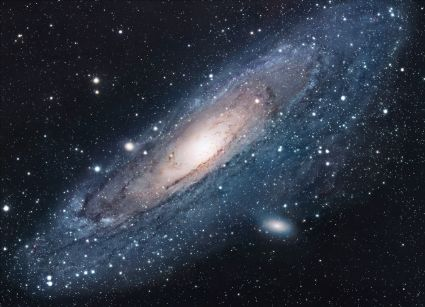
\includegraphics[scale=1.7]{universe}
\caption{The Universe}
\label{fig:universe}
\end{figure}

\section{Methods}
``I always thought something was fundamentally wrong with the universe'' \citep{adams1995hitchhiker}
\section{Results}

There is a plethora of tools to undertake GWAS in both eukaryotic and prokaryotic organisms, most tools are based on detecting SNVs whilst some also analyse the presence or absence of whole genes. However there has been, to our knowledge, no capacity to study structural variants beyond deletions using a GWAS framework. We therefore developed a suite of methods to process SV data into a format that is compatible with GWAS tools and then tested them on a dataset.






\subsection{Read depth based duplications as signals for GWAS}

As shown previously, read depth can be a reliable proxy for copy number. Therefore, the previously generated dataset, with a copy number assigned to each gene of each strain, was inputted to pySEER as a matrix. This was possible on pySEER as it can take a binary matrix, intended for the study of pangenomes, as input. However this meant that the CNV data had to be binary.


In order to use SVs as the ‘genotype’ in the ‘genotype-phenotype’ link that GWAS aims to establish, it was first necessary to prove the concept in a proof of concept experiment. To do this the strains containing duplications in Network 1 were given the phenotype of 1 and all other strains were given the phenotype of 0 in this perfect model phenotype.

%

\bibliographystyle{plain}
\bibliography{references}
\end{document}
